\documentclass[10pt,a4paper]{article}
\usepackage[utf8]{inputenc}
\usepackage[english]{babel}
\usepackage[T1]{fontenc}
\usepackage{amsmath}
\usepackage{amsfonts}
\usepackage{amssymb}
\usepackage{subcaption}
\usepackage{makeidx}
\usepackage{graphicx}
\usepackage{fourier}
\usepackage{listings}
\usepackage{color}
\usepackage{hyperref}
\usepackage[left=2cm,right=2cm,top=2cm,bottom=2cm]{geometry}
\author{Tommy Müller, Marcus Dittrich, Vincent Noculak}
\title{Rastertunnelmikroskopie}

\lstset{language=C++,
	keywordstyle=\bfseries\color{blue},
	commentstyle=\itshape\color{red},
	stringstyle=\color{green},
	identifierstyle=\bfseries,
	frame=single}
\begin{document}

\maketitle
\newpage
\tableofcontents
\newpage

\section{ Theoretische Vorbereitung}

Das Rastertunnelmikroskop ist eine Vorrichtung mit der sich Festkörperstrukturen in atomarer Größenordnung auflösen und graphisch darstellen lassen. Der Versuchsaufbau besteht prinzipiell aus einer, wenn möglich einatomigen Spitze, welche über ein piezoelektrisches Element bewegt werden kann und einer zu untersuchenden Probe. Zwischen Probe und Spitze wird über eine angelegte Spannung ein Tunnelstrom erzeugt, mit dem man die Oberflächenbeschaffenheit der Probe untersuchen kann.

\subsection{ Der quantenmechanische Tunneleffekt}

Der Tunneleffekt ist eine quantenmechanische Erscheinung, bei der ein Teilchen eine Potentialbarriere auch dann überwinden kann, wenn die Energie des Teilchens geringer ist als die Höhe der Barriere. Die Amplitude der Wellenfunktion nimmt dabei Exponentiell zur Breite der Barriere ab. Deswegen gilt, je geringer die Energie des Teilchens, desto geringer ist die Wahrscheinlichkeit des Tunnelns. Für den Zusammenhang zwischen Tunnelstrom, Abstand und angelegter Spannung lässt sich folgende Formel finden:
$I_{t} \sim V_{t} * e^{-c*\sqrt{\Phi }*s}$ ($\Phi$ - Austrittsarbeit in eV, s - Abstand in $\AA$  )

\subsection{	Piezoelektrischer Effekt}

Der piezoelektrische Effekt ist ein, bei Festkörpern auftauchendes Phänomen, bei dem eine mechanische Verformung eine Verschiebung des Ladugsschwerpunktes bewirkt, wodurch eine messbare Spannung induziert wird. Für die, in unserem Versuch verwendeten piezoelektrischen Elemente, wird der umgekehrte piezoelektrische Effekt verwendet. Hierbei führt das Anlegen einer Spannung zu einer Verformung des Festkörpers.

\subsection{	Rückkopplung und Regelkreistitle}

Als Regelkreis wird ein System bezeichnet, in dem der Abweichung einer physikalischen Größe über negative Rückkopplung entgegengewirkt wird. D.h. eine Änderung einer bestimmten physikalischen Größe führt zur proportionalen Änderung einer anderen Größe, welche an das Eingangssignal negativ gekoppelt ist. In unserem Versuchsaufbau wird beim Rastern über die, zu untersuchende Oberfläche, ein Regelkreis verwendet, um den Tunnelstrom konstant zu halten.

\subsection{	Tunnelspektroskopie}

Als Tunnelspektroskopie wird das Verfahren bezeichnet, bei dem Oberflächen einer Probe über den quantenmechanischen Tunneleffekt untersucht werden. Des Weiteren kann man Aussagen über die lokale elektronische Struktur des zu untersuchenden Stoffes treffen, da dem Prozess die Überlagerung von Elektronenzuständen zu Grunde liegt. Im Idealfall wird das Experiment unter Ultrahochvakuum Bedingungen durchgeführt, um das Ergebnis nicht zu verzerren.

\subsection{	Räumliche Struktur von Festkörpern}

Als Festkörper wird Materie im festen Aggregatzustand bezeichnet. Man unterscheidet dabei zwischen amorpher (ungeordnet) und kristalliner Ordnung ihrer Bausteine. Das, in unserem Versuch verwendete, Graphit weist eine hexagonale Gitterstruktur auf, welche in Basalschichten A und B zueinander, um einen festen Vektor verschoben, gestapelt sind. 

\subsection{	Elektronische Struktur einer Festkörperoberfläche}

Eine Festkörperoberfläche unterscheidet sich in ihren Eigenschaften zu denen im Inneren des Kristalls. Die Atome an der Grenzfläche versuchen in einen energetisch günstigeren Zustand zu gelangen, in dem sie ihre Bindungslänge zu tieferliegenden Schichten verringern. Dies führt zu einer Glättung der Oberflächendichte, was zu einer räumlichen um Ordnung der Oberflächenatome führen kann, wenn dadurch ein niedrigerer Energiezustand des Systems erreicht werden kann. Das führt dazu, das Elektronen an der Oberfläche schwächer gebunden sind.

\subsection{	Fourier Transformation}

Die Fourier Transformation ist ein unitäres Verfahren, bei dem zwischen Orts- und Impulsraum bzw. Zeit und Frequenzraum transformiert wird. Das Verfahren ist in beide Richtungen verlustfrei.

\section{	Versuchsaufbau}

Das, in unserem Versuch verwendete Raster-Tunnelmikroskop ist ein Eigenbau der Arbeitsgruppe und arbeitet unter atmosphärischem Druck. Die Bewegung des Messkopfes in X-Y-Z-Richtung wird über einen PC mit der Freeware WSxM der Firma Nanotec gesteuert. Die Z-Richtung des Messkopfes wird über einen Regelkreis variiert, bei konstantem Tunnelstrom. Dieser Messkopf besteht im Wesentlichen aus einem Piezo-Röhren-Scanner und einer Messspitze aus einer Titan-Iridium Legierung. Der gesamte Versuchsaufbau wurde auf einem schwingungsgedämpften Tisch installiert, um Messfehler durch Vibrationen zu minimieren.

\begin{figure}[h]
	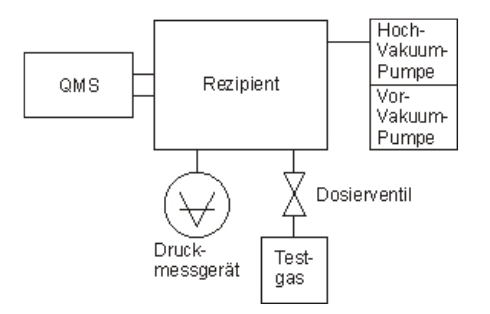
\includegraphics[scale = 0.5]{aufbau.png}
	\centering
	\caption{Aufbau des Raster-Tunnelmikroskops}
	\label{diagramm_aufspaltung}
\end{figure}

\section{Durchführung}

Bevor Messungen am Versuchsaufbau durchgeführt werden können müssen die Messspitze und die zu untersuchende Graphitoberfläche präpariert werden. Dafür wurde die alte Messspitze zunächst aus dem Aufbau entfernt und mit einer Zange so abgekniffen, das eine möglichst dünne Spitze erzeugt wurde. Des Weiteren wurde mit einer Lage Tesafilm die oberste Schicht der Graphitprobe entfernt, um mögliche Verunreinigungen zu entfernen. Anschließend haben wir die Spitze wieder in den Messkopf eingesetzt und mittels einer Mikrometerschraube per Hand an die Probe angenähert. Mit Hilfe eines Schrittmotors wurde die Spitze dann bis auf wenige $\AA$ angenähert, bis ein vorher festgelegter Tunnelstrom messbar war. Danach wurde der Motor abgenommen und die Schutzglocke aufgesetzt. Danach haben wir verschiedene Messungen mit Variationen der Parameter, wie z.B. der angelegten Bias Spannung (zwischen Probe und Spitze) oder des festgelegten Tunnelstroms gemacht, um möglichst gute Aufnahmen der Graphit-Oberfläche zu bekommen. Atomare Auflösung konnten wir dabei allerdings nicht erreichen.

\subsection{Parameter}

Zunächst wurde der Messaufbau, wie in der Durchführung beschrieben hergerichtet. Zum Annähern der Spitze mithilfe des Schrittmotors wurden die Einstellungen aus Abbildung \ref{parameter} im Menü DA ausgewählt. Wichtige Parameter sind Size, Speed, Bias, Set Point, Z Gain und der Logarithmic Feedback. Size bestimmt die Kantenlänge der untersuchten Probenoberfläche in nm und der Parameter Speed gibt die Scangeschwindigkeit einer Linie in s an. Bias beschreibt die angelegte Probenspannung in mV und Set Point charakterisiert den konstanten Tunnelstrom während der Messung. Der Z-Gain ist die eingestellte Hochspannungsverstärkung für die Z-Bewegung. Die Funktion des Logarithmic Feedbacks besteht darin, die Messungergebnisse während der Bewegung zu stabilisieren. Sind Proportional und Integral Gain zu niedrig eingestellt, kommt der Messkopf nicht hinterher und die Messung verschwimmt, ist der Gain zu hoch eingestellt, kann es zu Oszillationen kommen. 

\begin{figure}[h]
	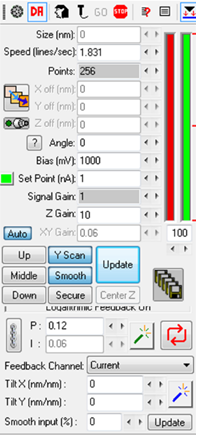
\includegraphics[scale = 0.9]{parameter.png}
	\centering
	\caption{Approachsettings des RTM}
	\label{parameter}
\end{figure}

\section{Versuchsauswertung}

\subsection{Vermessung von Graphit }

\subsubsection{ Kantenhöhen}

Als ersten haben wir uns mit der Funktionsweise des Rastertunnelmikroskops vertraut gemacht und im Verlauf der Zeit 79 Bilder gemacht haben. 
Diese Bilder haben wir anschließend nach und nach angeguckt und leider nur 16 Kanten vermessen können. Alle Bilder haben wir mit dem Tool WSxM 4.0 Beta 8.2 vermessen. 
Die Funktion "Local plane" und "profile" nutzen wir bei den Bildern. Anschließend wurde eine Linie gezogen und dann ein Höhenprofil gezeigt. (Siehe Bilder der Kanten unten)
Viele Bilder waren fehlerhaft und konnten nicht zur Bestimmung von Kantenhöhen verwendet werden.



\subsubsection{Bilder von 10 Kanten}

\begin{figure}[]
	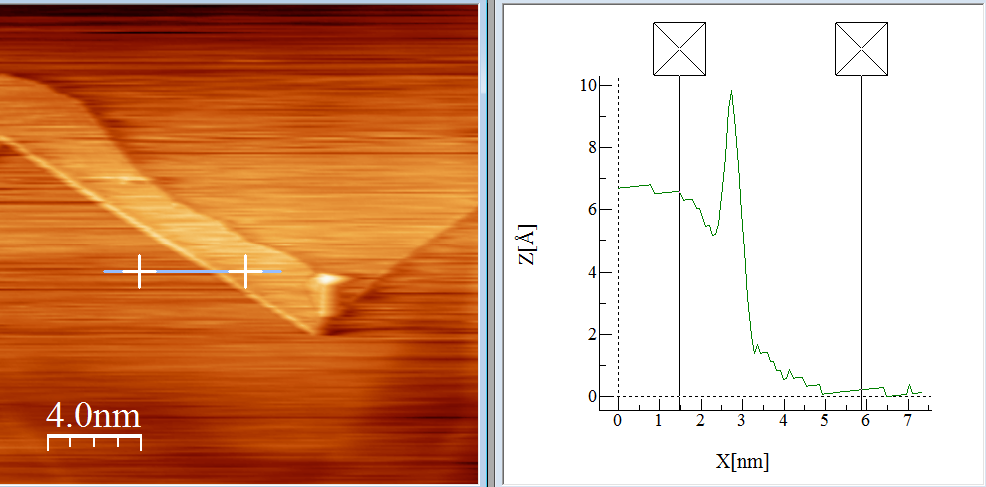
\includegraphics[scale = 0.2]{bild00.png}
	\centering
	\caption{Bild 0 Kante 0.637 nm}
	\label{b0}
\end{figure}

\begin{figure}[]
	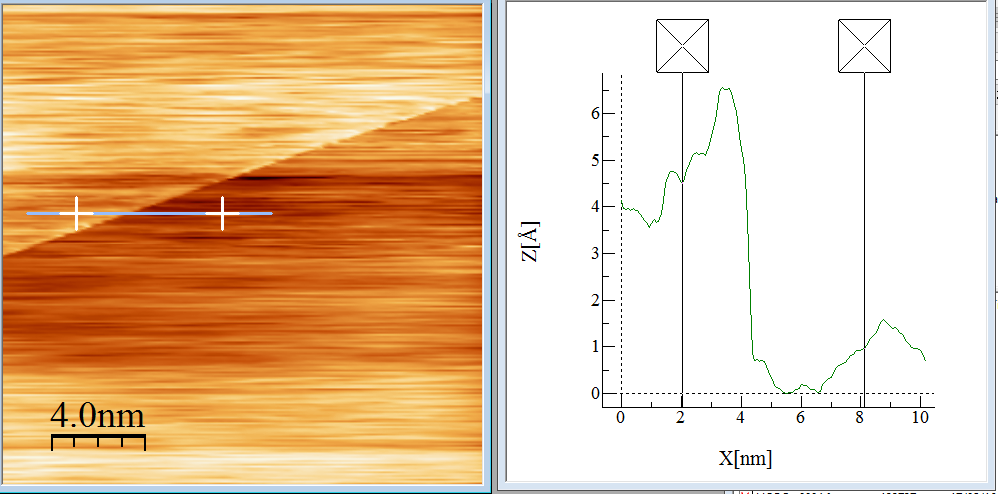
\includegraphics[scale = 0.2]{bild11.png}
	\centering
	\caption{Bild 11 Kante 0.353 nm}
	\label{b11}
\end{figure}
\begin{figure}[]
	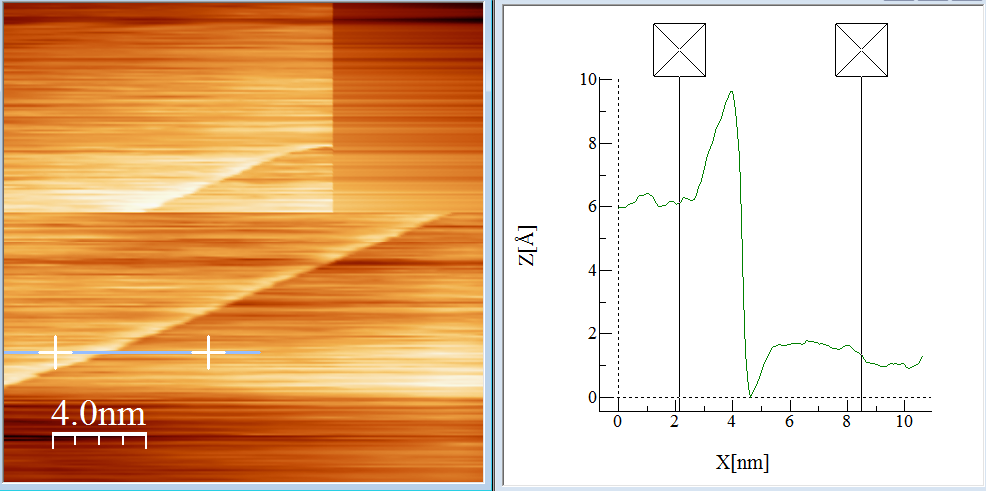
\includegraphics[scale = 0.2]{bild12.png}
	\centering
	\caption{Bild 12 Kante 0.447 nm}
	\label{b12}
\end{figure}

\begin{figure}[]
	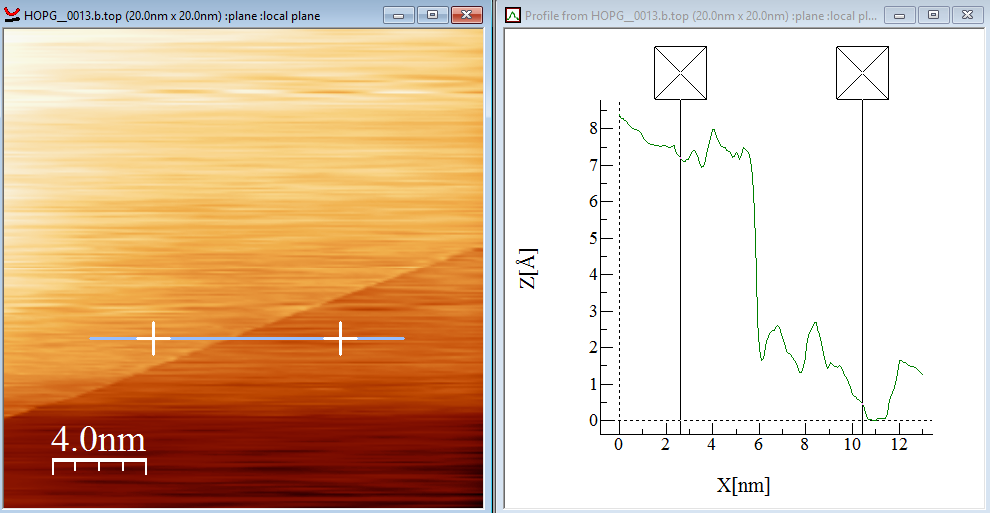
\includegraphics[scale = 0.2]{bild13.png}
	\centering
	\caption{Bild 13 Kante 0.677 nm}
	\label{b13}
\end{figure}

\begin{figure}[]
	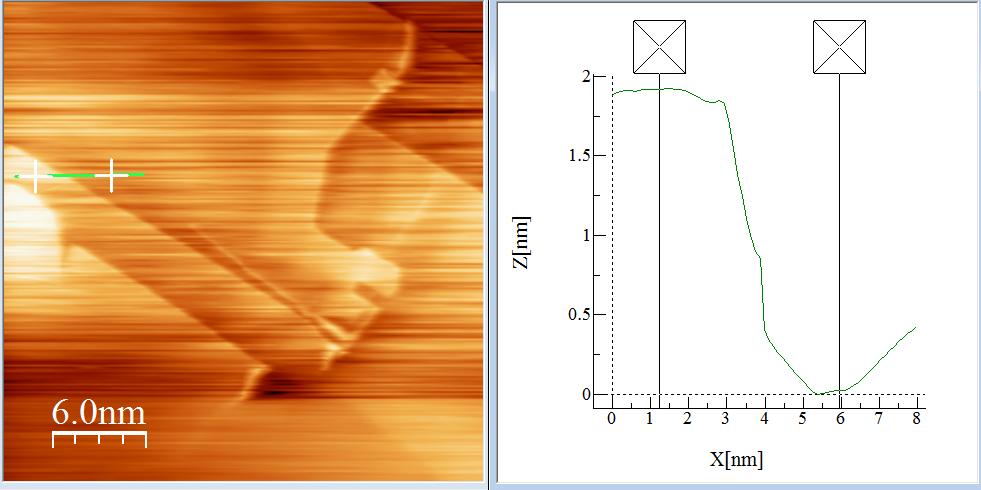
\includegraphics[scale = 0.2]{bild23.png}
	\centering
	\caption{Bild 23 Kante 1.896 nm}
	\label{b23}
\end{figure}
\begin{figure}[]
	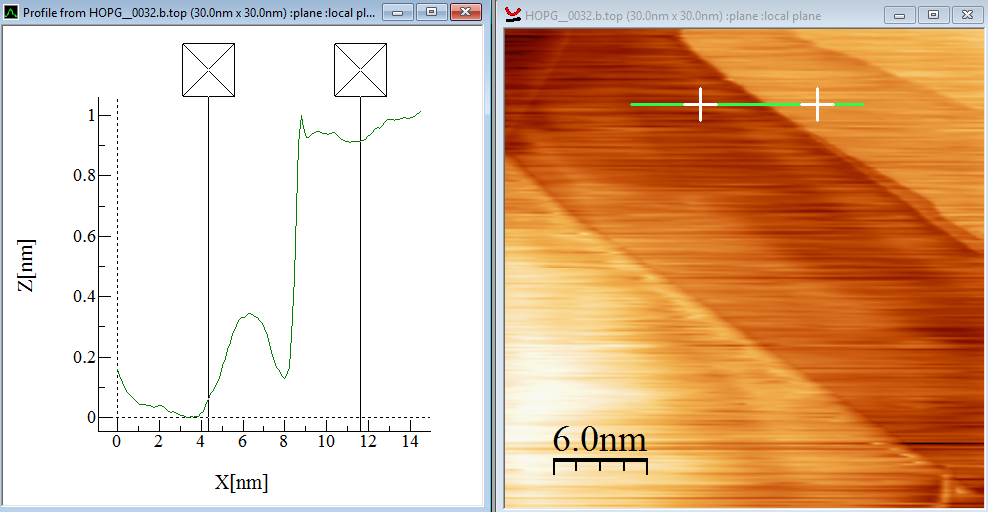
\includegraphics[scale = 0.2]{bild32.png}
	\centering
	\caption{Bild 32 Kante 0.853 nm}
	\label{b32}
\end{figure}

\begin{figure}[]
	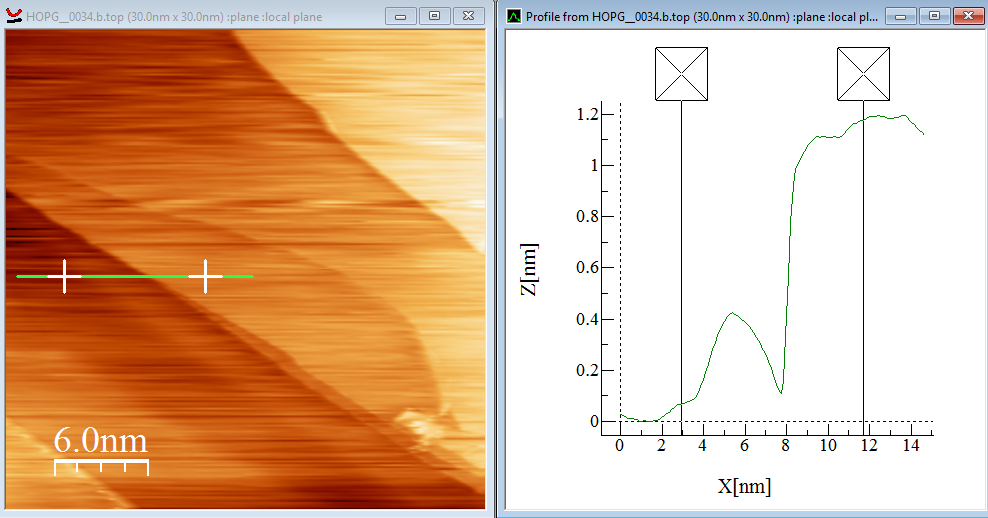
\includegraphics[scale = 0.2]{bild34.png}
	\centering
	\caption{Bild34 Kante 1.103 nm}
	\label{b34}
\end{figure}


\begin{figure}[]
	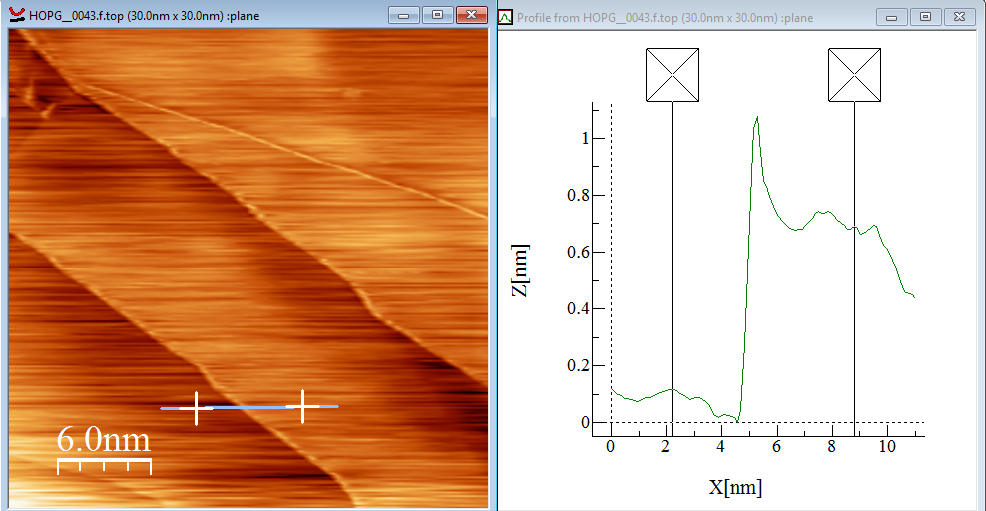
\includegraphics[scale = 0.2]{bild43.png}
	\centering
	\caption{Bild 43 Kante 0.572 nm}
	\label{b43}
\end{figure}

\begin{figure}[]
	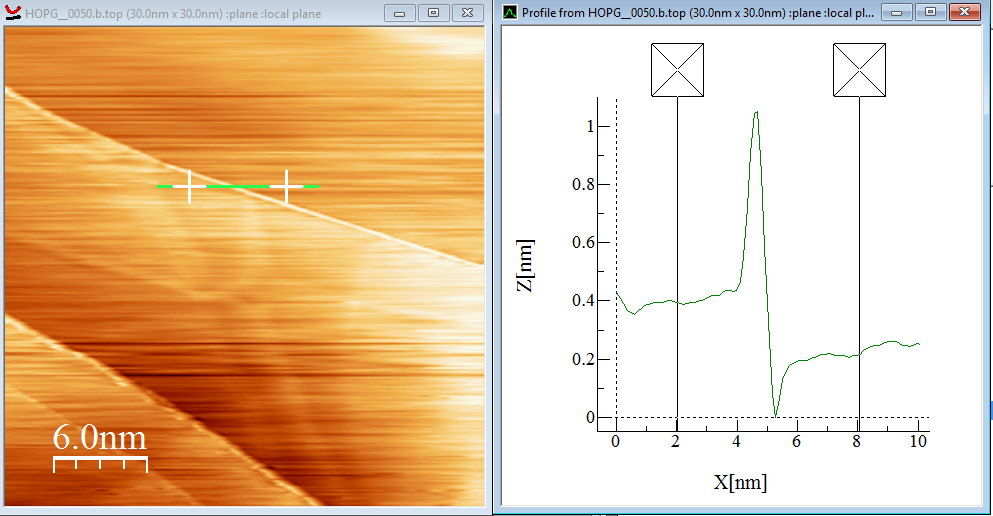
\includegraphics[scale = 0.2]{bild50.png}
	\centering
	\caption{Bild 50 Kante 0.179 nm}
	\label{b50}
\end{figure}

\begin{figure}[]
	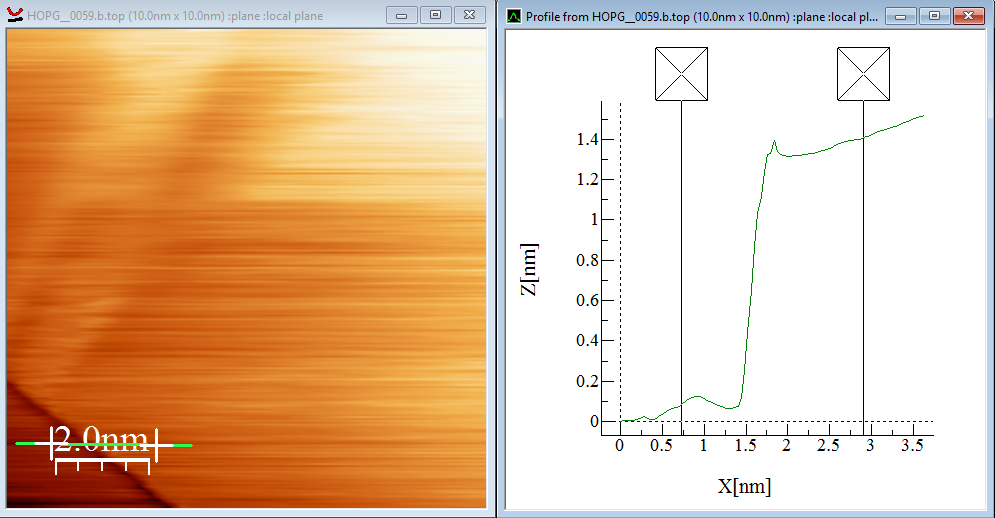
\includegraphics[scale = 0.2]{bild59.png}
	\centering
	\caption{Bild 59 Kante 1.302 nm}
	\label{b59}
\end{figure}

Nach dem wir alle Kanten vermessen haben, ordneten wir diese der Höhe nach. Die Höhen gingen von 0.179 nm bis 1.896 nm. Im folgenden haben wir die Höhen in einem Diagramm abgetragen und die theoretischen Kanten mit den roten Linien markiert.

\begin{figure}[]
	\includegraphics[scale = 0.5]{khglist.png}
	\centering
	\caption{Liste der ordeneten Kanten}
	\label{list}
\end{figure}

\begin{figure}[]
	\includegraphics[scale = 0.5]{khgdia.png}
	\centering
	\caption{Diagramm Höhe der Kanten sowie in Rot Theoretische Kantenhöhen}
	\label{list}
\end{figure}

In dem Diagramm zu den Höhen sehen wir eine Ansammlung von Kanten bei den N = 2 und 4 diese Kanten werden am besten durch unsere Messungen repräsentiert. Die anderen theoretischen Kanten werden nur bedingt durch unsere Messergebnisse wiedergespiegelt.
Beim Vergleichen der theoretischen Kanten mit dem Messergebissen muss drauf geachtet werden das die Kanten auch reale Kanten sind und keine Missinterpretation der Software. Die Form der Spitze ist auch entscheidend ob die Kanten "gut" erkennbar sind. Bei einigen Bildern waren die "Kanten" eher gebogen und dies kann bei einem Kristall nicht sein.

\subsection{Ebene Grafitoberfläche}

Wir sollten eine Ebene Fläche im Grafit finden und versuchen anhand dieser die Atomare Struktur des Grafits darzustellen. Obwohl wir Ebene Flächen im Grafit fanden, war es nicht möglich Atomare Strukturen zu erkennen. Dies lag wahrscheinlich daran, dass die Spitze unseres Sensors nicht spitz genug war. Deshalb haben wir zur Untersuchung der Atomaren Struktur die Daten aus den Referenzmaterialien genommen. Die Messung aus den Referenzmaterialien kann in \ref{Grafitoberflächenebene} gesehen werden. Hier ist \ref{grafob1} die rohe Messung an sich. In \ref{grafob2} haben wir mithilfe einer doppelten Fouriertransformation Störung aus der Messung entfernt. Dadurch lässt sich sie atomare Struktur genauer erkennen und untersuchen.

\begin{figure}[h]
	\centering
	\begin{subfigure}{0.45\textwidth}
		\centering
		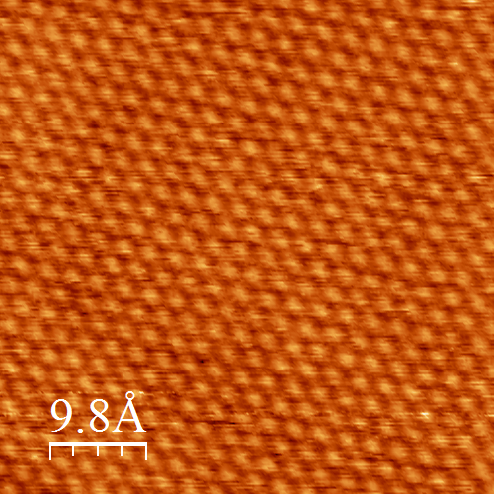
\includegraphics[width=\textwidth]{vor_doppelter_fourier.png}
		\caption{gemessene Grafitoberfläche}
		\label{grafob1}
	\end{subfigure}
	\begin{subfigure}{0.45\textwidth}
		\centering
		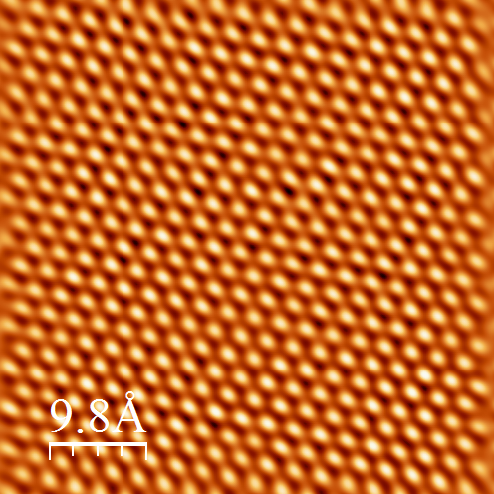
\includegraphics[width=\textwidth]{nach_doppelter_fourier.png}
		\caption{Gemessene Grafitoberfläche, nachdem Störungen durch eine doppelte Fouriertransformation beseitigt wurden}
		\label{grafob2}
	\end{subfigure}

	\caption{Messung des Tunnelstroms an einer ebenen Fläche Grafit}
	\label{Grafitoberflächenebene}
\end{figure}

Es kann klar erkannt werden, dass die Kohlenstoffatome regelmäßig in einer Kristallstruktur angeordnet sind. Man erkennt ein hexagonales Kristallsystem, wie es für Grafit zu erwarten war.

\begin{figure}[h]
	\centering

	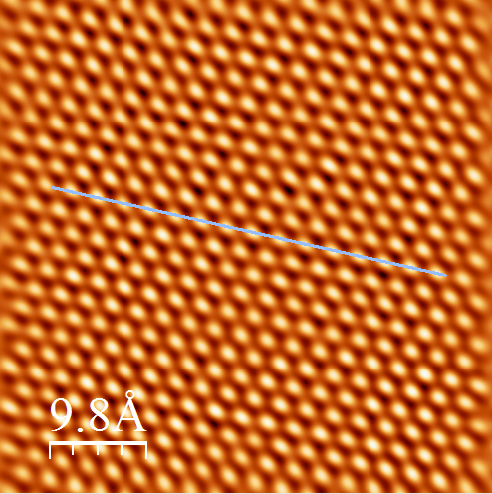
\includegraphics[scale = 0.6]{Aufnahme_Ebene_doppelte_fourier2.png}

	\caption{Messung der Abstände der atomaren Erhebungen}
	\label{Messungerh1}
\end{figure}

Entlang der in \ref{Messungerh1} zu sehenden Linie haben wir die Abstände der atomaren Erhebungen gemessen. Das dazugehörige Diagramm kann in Abbildung \ref{Messungerh2} gesehen werden. Wir haben alle Abstände entlang der zu sehenden Gerade gemessen und anschließend einen Mittelwert mit Standartabweichung gebildet. Die gemessenen Abstände sind in Tabelle \ref{Messungerh5} zu sehen. Unser Wert für den Abstand der atomaren Erhebungen ist $(0,266 \pm 0,001) nm$.

Laut der Theorie sehen wir in dem mit dem Rastertunnelmikroskop aufgenommenen Bild nur jedes zweite Atom des Grafit-Kristalls. Der planare Abstand nächster Nachbarn im Kristall ist mit $b = 0,142 nm$ gegeben. Der von uns zu erwartende Abstand der atomaren Erhebungen lässt sich mithilfe des Kosinussatzes als 

\begin{equation}
	s = b \cdot \sqrt{2(1-cos(120^\circ))} = 0,246 nm
\end{equation}

berechnen. Auch wenn unserer gemessener Wert bis zur ersten signifikanten Stelle mit diesem theoretischen Wert übereinstimmt, liegt dieser wegen der kleinen Standartabweichung nicht innerhalb des dritten Fehlerintervalls. Dass unser Wert nicht mit dem theoretischen Übereinstimmt, könnte daran liegen, dass wir mit dem Rastertunnelmikroskop nicht senkrecht auf die Probe gucken. Dadurch werden bei der Messung Abstände zwischen atomaren Erhebungen verzerrt.

\begin{figure}[h]
	\centering
	
	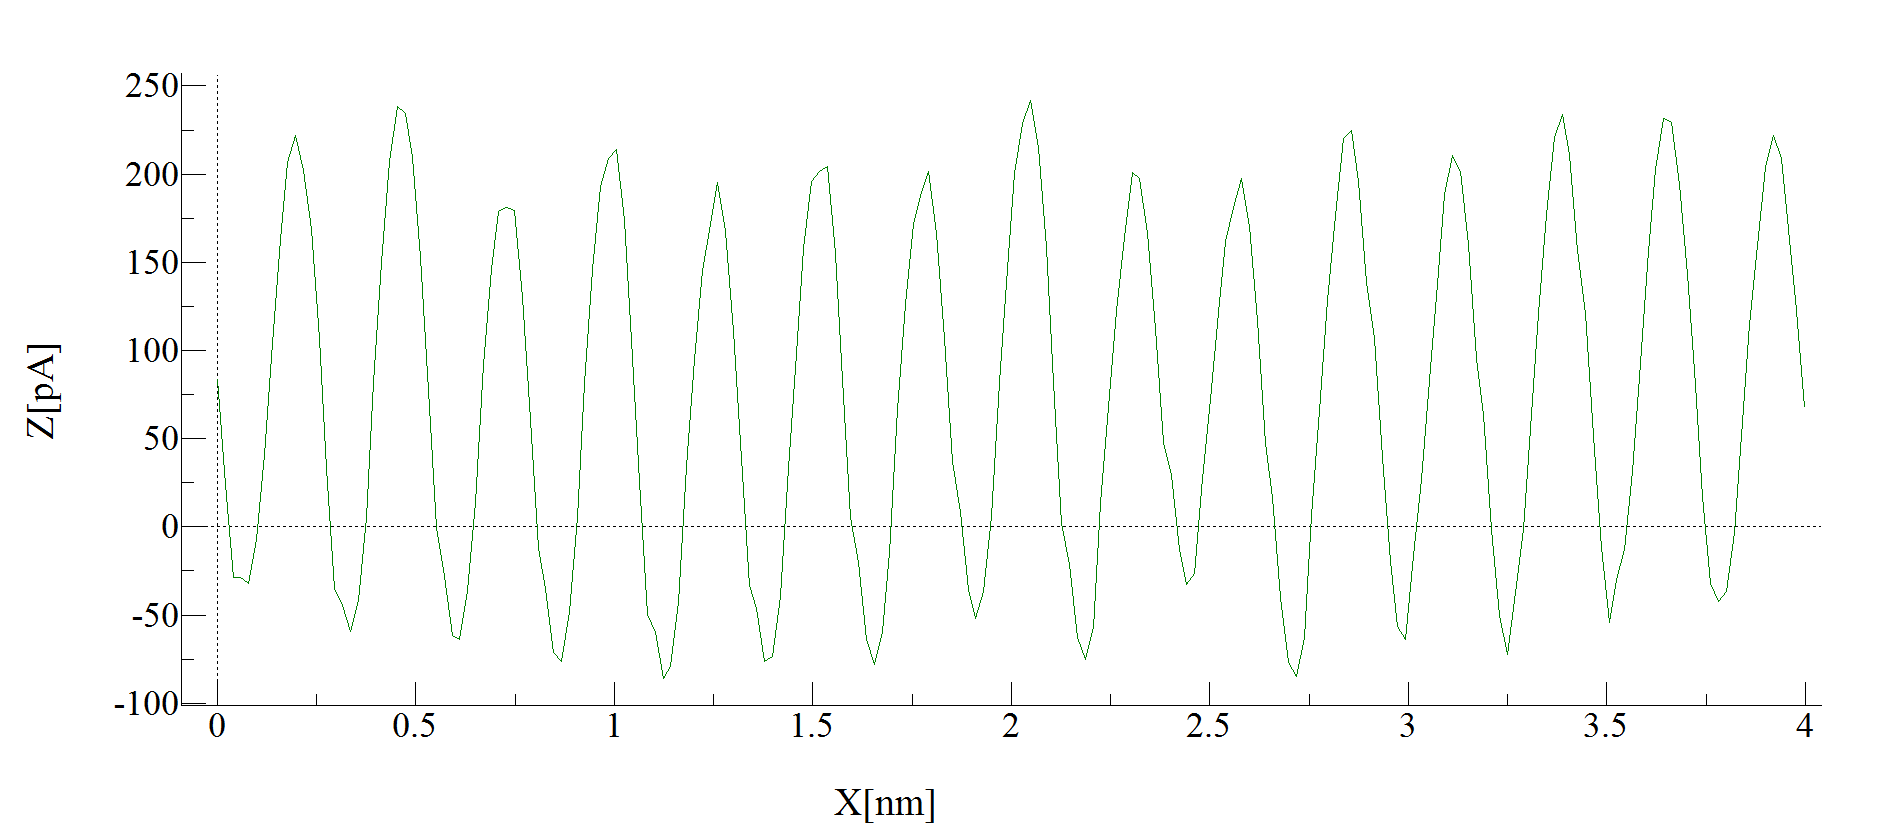
\includegraphics[scale = 0.3]{Aufnahme_Ebene_doppelte_fourier.png}
	
	\caption{Diagramm zur Messung der Abstände der atomaren Erhebungen}
	\label{Messungerh2}
\end{figure}

Zur Messung der Höhe der atomaren Erhebungen mussten wir die Messdaten, die die Höhen und nicht den Tunnelstrom angeben verwenden. Auf diesen Messdaten waren die atomaren Erhebungen selbst nach einer doppelten Fouriertransformation nicht sehr klar zu erkennen, wie in Abbildung \ref{Messungerh3} zu sehen ist. Wir haben entlang der in Abbildung \ref{Messungerh3} zu sehenden Geraden gemessen. Das zu der Geraden gehörende Diagramm kann in \ref{Messungerh4} gesehen werden. An diesem Diagramm haben wir durch das Bilden der Differenz von Maxima und Minima die Höhen der atomaren Erhebungen gemessen. Die Werte können in Tabelle \ref{Messungerh5} gesehen werden. Nach dem Bilden eines Mittelwerts und einer Standardabweichung haben wir für den Wert der Höhe $(8,8 \pm 0,4) pm$.

Der theoretische Wert für den Abstand benachbarter Ebenen in Grafit ist $335 pm$. Dieser Wert übersteigt bei weitem die von uns gemessene Höhe der atomaren Erhebungen. Folglich lassen sich unsere gemessenen Höhen nicht mit diesem Wert identifizieren. Um nachzuvollziehen, wie unsere gemessenen Höhen für die atomaren Erhebungen zustande kommen, müssen wir die Form der Metallspitze, die wir als Sensor benutzen, mit in Betracht ziehen. Diese Spitze hat einen gewisses Ausmaß und kann, wenn es als äußerstes Orbital ein s-Orbital hat, als eine Kugel mit gewissen Radius verstanden werden. Lässt der Tunnelstrom zwischen Sensor und Probe nach, fährt dieser näher an die Probe ran. Dies ist zum Beispiel zwischen den atomaren Erhebungen der Fall. Weil die Metallspitze jedoch einen Radius hat wird es auch, wenn es über einer Stelle zwischen den atomaren Erhebungen ist, mit diesen beim Versuch sich der Probe anzunähern "zusammenstoßen". Deshalb sind die gemessenen Höhen der atomaren Erhebungen viel kleiner als der tatsächliche Ebenenabstand.

\begin{figure}[h]
	\centering
	
	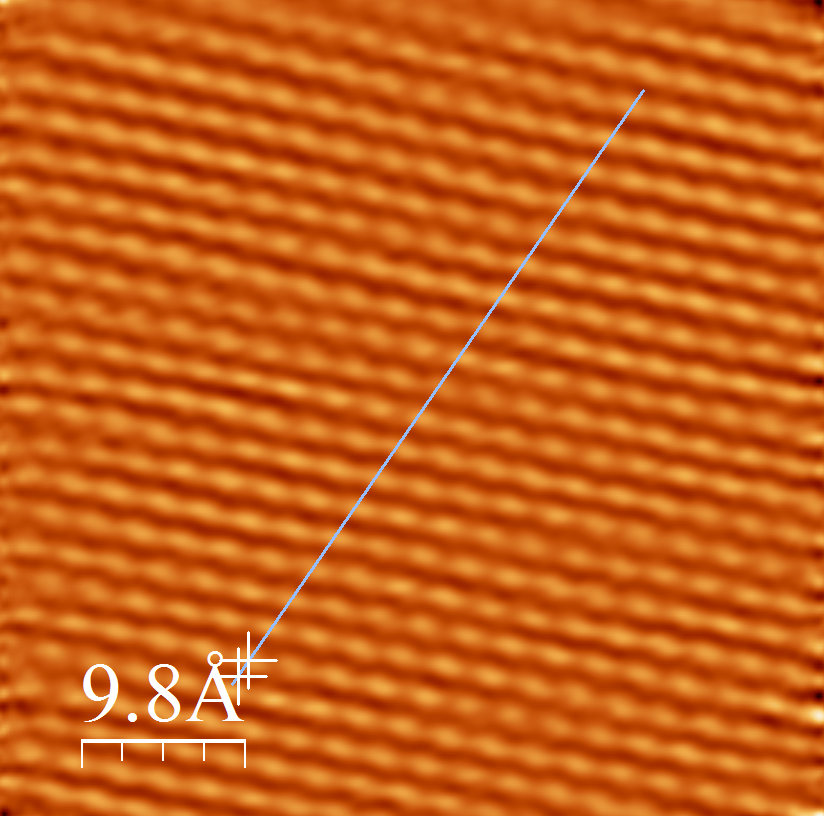
\includegraphics[scale = 0.4]{hohenmessung11.png}
	
	\caption{Messung der Höhe der atomaren Erhebungen}
	\label{Messungerh3}
\end{figure}

\begin{figure}[h]
	\centering
	
	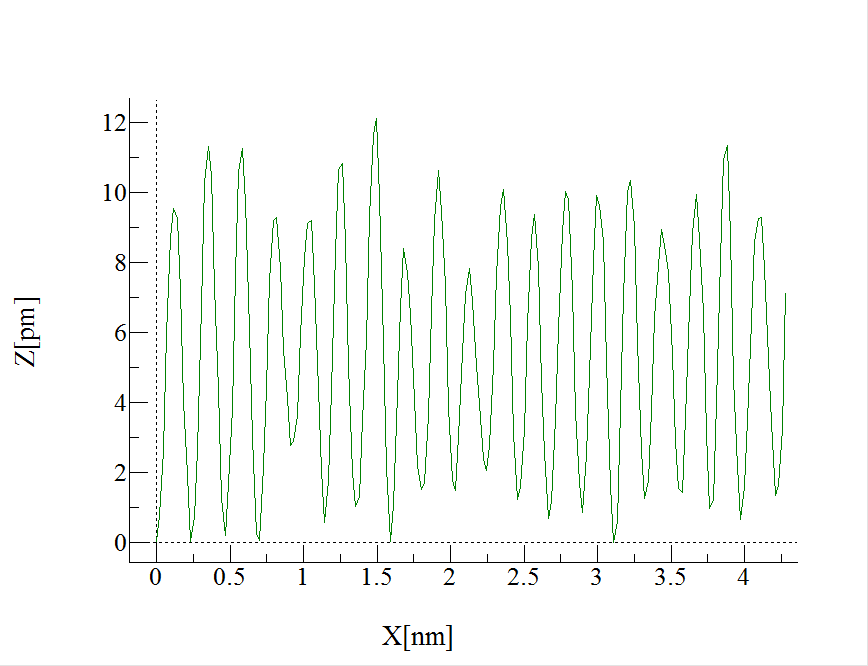
\includegraphics[scale = 0.7]{hohenmessung1_diagramm.png}
	
	\caption{Diagramm zur Messung der Höhe der atomaren Erhebungen}
	\label{Messungerh4}
\end{figure}

\begin{table}[h!]
	\centering
	\begin{tabular}{|l|r|c|lrp{16cm}}\hline
		Abstand/nm & Höhe/pm\\\hline
		0,262 & 9,364 \\
		0,27 & 10,901 \\
		0,264 & 10,967\\
		0,259& 6,444 \\
		0,259 & 8,436 \\
		0,267 & 9,675 \\
		0,264 & 11,881\\
		0,27 & 6,705\\
		0,262 & 9,023\\
		0,27 & 5,687\\
		0,262 & 8,74\\
		0,277 & 8,513\\
		0,262 & 8,829\\
		0,27 & 9,606\\
		& 8,773\\
		& 7,371\\
		& 8,671\\
		& 10,187\\
		& 7,835\\
		\hline
	\end{tabular}
	\caption{Gemessene Werte für die Abstände und Höhen der atomaren Erhebungen}
	\label{Messungerh5}
\end{table}

Anhand von Abbildung \ref{Messungerh6} haben wir die Winkel zwischen den atomaren Richtungen gemessen. Unsere gemessenen Winkel, startend von dem Winkel rechts oben und dann entgegen dem Uhrzeigersinn laufend sind $63^\circ$, $67^\circ$, $48^\circ$, $67^\circ$, $66^\circ$ und $49^\circ$, mit jeweils einem Fehler von $1^\circ$. Wegen der hexagonalen Struktur von Grafit wäre bei einer naiven Herangehensweise zu erwarten, dass alle Winkel $60^\circ$ sind. Dies ist nicht der Fall. Es fällt auf dass die besonders kleinen Winkel($48^\circ$ und $49^\circ$) entgegengesetzt voneinander liegen. Die unterstützt die Theorie, dass die Winkel deshalb alle unterschiedlich groß sind, weil wir nicht senkrecht auf die Grafitprobe gucken.

 Eine andere Erklärung für die unterschiedlichen Winkel könnte daran liegen, dass der Sensor in einem Raster über die Probe fährt. Dabei könnte es zu einem Umrechnungsfehler bei der Berechnung des Bildes aus den Rasterpunkten kommen. Wir halten diese Theorie als weit unwahrscheinlicher, als die, dass wir nicht senkrecht auf die Probe gucken.
 
 Weil von uns beobachteten atomaren Erhebungen der Grafits bilden ein hexagonales Kristallgitter. Es ist 6-zählig. Entlang einer Translation von ganzzahligen Abständen der atomaren Erhebungen der in \ref{Messungerh6} eingezeichneten Linien, gibt es außerdem eine Tanslationssymmetrie. Zusätzlich sieht man, dass bei einer Spiegelung entlang einer der Geraden und einer Inversion an dem Punkt, in dem sich die Geraden schneiden, das Gitter symmetrisch ist.

\begin{figure}[h]
	\centering
	
	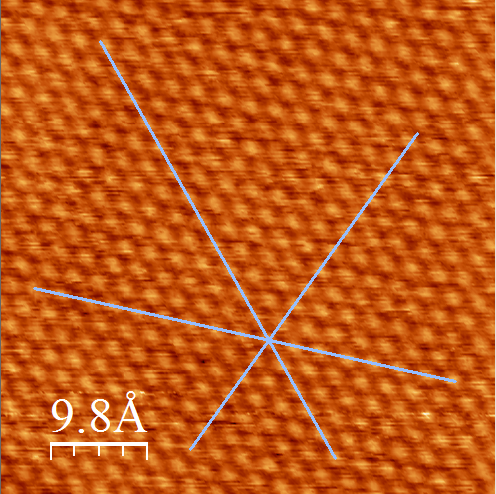
\includegraphics[scale = 0.7]{Winkelmessung_kristall.png}
	
	\caption{Messung der Winkel zwischen den atomaren Richtungen}
	\label{Messungerh6}
\end{figure}

\subsection{Fouriertransformation einer ebenen Fläche Grafits}

In Abbildung \ref{fouriertansformation_ebene} kann das Gitter aus Abbildung \ref{grafob1} nach einer Fouriertransformation betrachtet werden. Man erkennt sechs Punkte, die auf einem leicht verzerrten Hexagon um den Ursprung liegen. Um den Ursprung herum sieht man Werte in geringer Intensität. Dies sind die Störungen, die beim Aufnehmen der Messung entstanden sind. Die sechs zu erkennenden Punkte beinhalten alle Informationen über die Periodizität den gemessenen Gitters. Jedem der sechs Punkte kann ein Vektor $\vec{k}$ zugeordnet werden. Dies ist ein Wellenvektor, der eine Periodizität des Gitter angibt. Verschiebt man das Gitter also um eine Periode der Welle, die mit dem Wellenvektor $\vec{k}$ zu assoziieren ist, bleibt das Gitter unverändert. Daraus lässt sich leicht folgern, dass man aus $\vec{k}$ direkt den Abstand zweier atomarer Erhebungen berechnen kann durch.

\begin{equation}
	|k| = \frac{2\pi}{a}
	\label{formelk}
\end{equation}

Hier ist a der Abstand zweier atomarer Erhebungen

\begin{figure}[h]
	\centering
	
	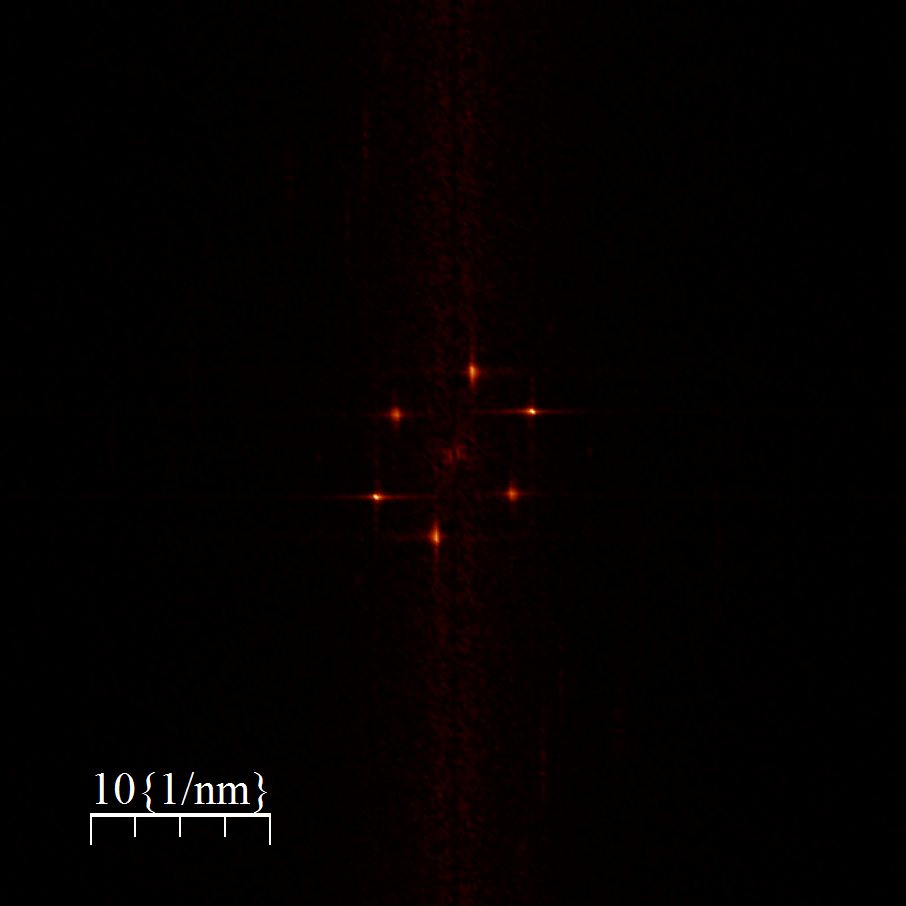
\includegraphics[scale = 0.5]{Fouriertrasformation_kristall.png}
	
	\caption{Fouriertransformation von Abbildung \ref{grafob1}}
	\label{fouriertansformation_ebene}
\end{figure}

\section{Diskussion}

Wir haben mit dem Rastertunnelmikroskop die Struktur von Grafit betrachtet. Da unsere Sensorspitze nicht fein genug war konnten wir zwar Kanten an der Oberfläche erkennen, die atomare Struktur des Grafits konnten wir jedoch nicht erkennen, beziehungsweise nur eingeschränkt über eine kleine Fläche. Deshalb mussten wir zur Betrachtung der Struktur von Grafit Referenzdaten benutzen.

Anhand der Referenzdaten konnten wir die hexagonale Struktur des Grafits erkennen. Es konnten Translations-, Inversions-, Spiegelungs- und Rotationssymmetrien erkannt werden. Die leicht unterschiedlichen Größen der Winkel zwischen den atomaren Richtungen konnten wir damit erklären, dass das Rastertunnelmikroskop nicht senkrecht auf die Grafitprobe schaute. Obwohl es uns gut gelang, die Struktur des Grafits zu untersuchen, konnten wir keine mit dieser Struktur zusammenhängenden physikalischen Größen, wie zum Beispiel den Abstand der Kohlenstoffatome oder den Ebenenabstand, im Einklang mit der theoretischen Werten bestimmen. Unser Wert für den Abstand der atomaren Erhebungen war $(0,266 \pm 0,001) nm$ und wich mit 20 Fehlerintervallen von dem theoretischen Wert von $0,246 nm$ ab.

Anhand der Fouriertransformation (Abb. \ref{fouriertansformation_ebene}) konnte die periodische Struktur des Grafitgitters eindeutig dargestellt werden. Möglicherweise ist die fouriertransformierte Darstellung des Gitters besser als das direkte Abmessen an der Gitterstruktur geeignet, um die Abstände der atomaren Erhebungen zu bestimmen. Um dies zu tun müsste das Rastertunnelmikroskop möglich senkrecht auf das Grafit schauen, damit die periodischen Strukturen des Gitters nicht verzerrt werden. Es wäre auch möglich diese Verzerrung numerisch zu lösen, was jedoch mit hohem Aufwand verbunden wäre. Die atomaren Abstände könnten dann unter Verwendung von \ref{formelk} mit dem in der Fourierdarstellung vorkommenden $k$ berechnet werden.

Um bessere Versuchsergebnisse zu erzielen, könnte man die Sensorspitze des Rastertunnelmikroskops mit einer anderen Methode herstellen. Die Feinheit der Sensorspitze ist für den Erfolg des Versuchs ausschlaggebend und bestimmt, ob es Möglich sein wird, die atomare Struktur des Grafits zu messen.

Zum Messen der Stufen auf der Grafitoberfläche konnten wir unsere eigenen Messbilder benutzen. Das vermessen der Bilder ergab nur 16 Kanten. Diese Kanten sind nach der Höhe geordnet und im Diagramm 12 zu sehen. Wir konnten mit unseren Messergebnissen die theoretischen Kanten relativ gut darstellen. Vor allem den zweifachen und vierfachen Netzebenenabstand können unsere Messergebnisse rekonstruieren. Einige Messergebisse sind fast genau zwischen zwei Ebenen, dies könnte an der schlechte Wahl von Messpunkten am Bild liegen. Eine vorab Sondierung der Bilder wäre von Nöten gewesen mehr Kanten zu erfasst und die Ergebnisse klarer zu gestalten.

\end{document}